% ============================================================
% Figure snippet template (put this in figures/<stem>.tex)
%
% Purpose:
% - Keep figures modular and easy to insert exactly where first mentioned.
% - Enforce a consistent naming/labeling convention across the project.
%
% Recommended workflow:
% 1) Create figures/<stem>.pdf
% 2) Create figures/<stem>.tex (this file) with the same <stem>
% 3) In the manuscript, cite then input the figure at first mention:
%      ... Figure~\ref{fig:<stem>}.%
%      \input{figures/<stem>.tex}
%    The percent sign (%) prevents LaTeX from inserting an extra space/newline
%    between the sentence and the \input command when you keep them adjacent.
%
% Conventions (highly recommended):
% - File stem: use only letters, digits, underscore, or hyphen.
%   Avoid spaces and punctuation in stems (e.g., avoid ".", "()", "/", ",").
% - PDF and TEX stems match:
%     figures/example1.pdf  <->  figures/example1.tex
% - Label matches the stem with a prefix:
%     \label{fig:example1}
% - Label characters: use only [A-Za-z0-9:_-]. Avoid special characters.
%
% Float placement:
% - Default: [!t] (strong preference for top of page; standard for manuscripts).
% - If you need the figure to appear immediately after a section heading
%   (common for the first figure in an appendix section), use [!h] in that file.
%   Note: figures are floats; LaTeX may still move them if necessary.
% ============================================================

\begin{figure}[!t]
  \centering

  % Graphics:
  % - Prefer \textwidth (not 1\textwidth) as it is the conventional form.
  % - Use a relative width so figures scale correctly if margins change.
  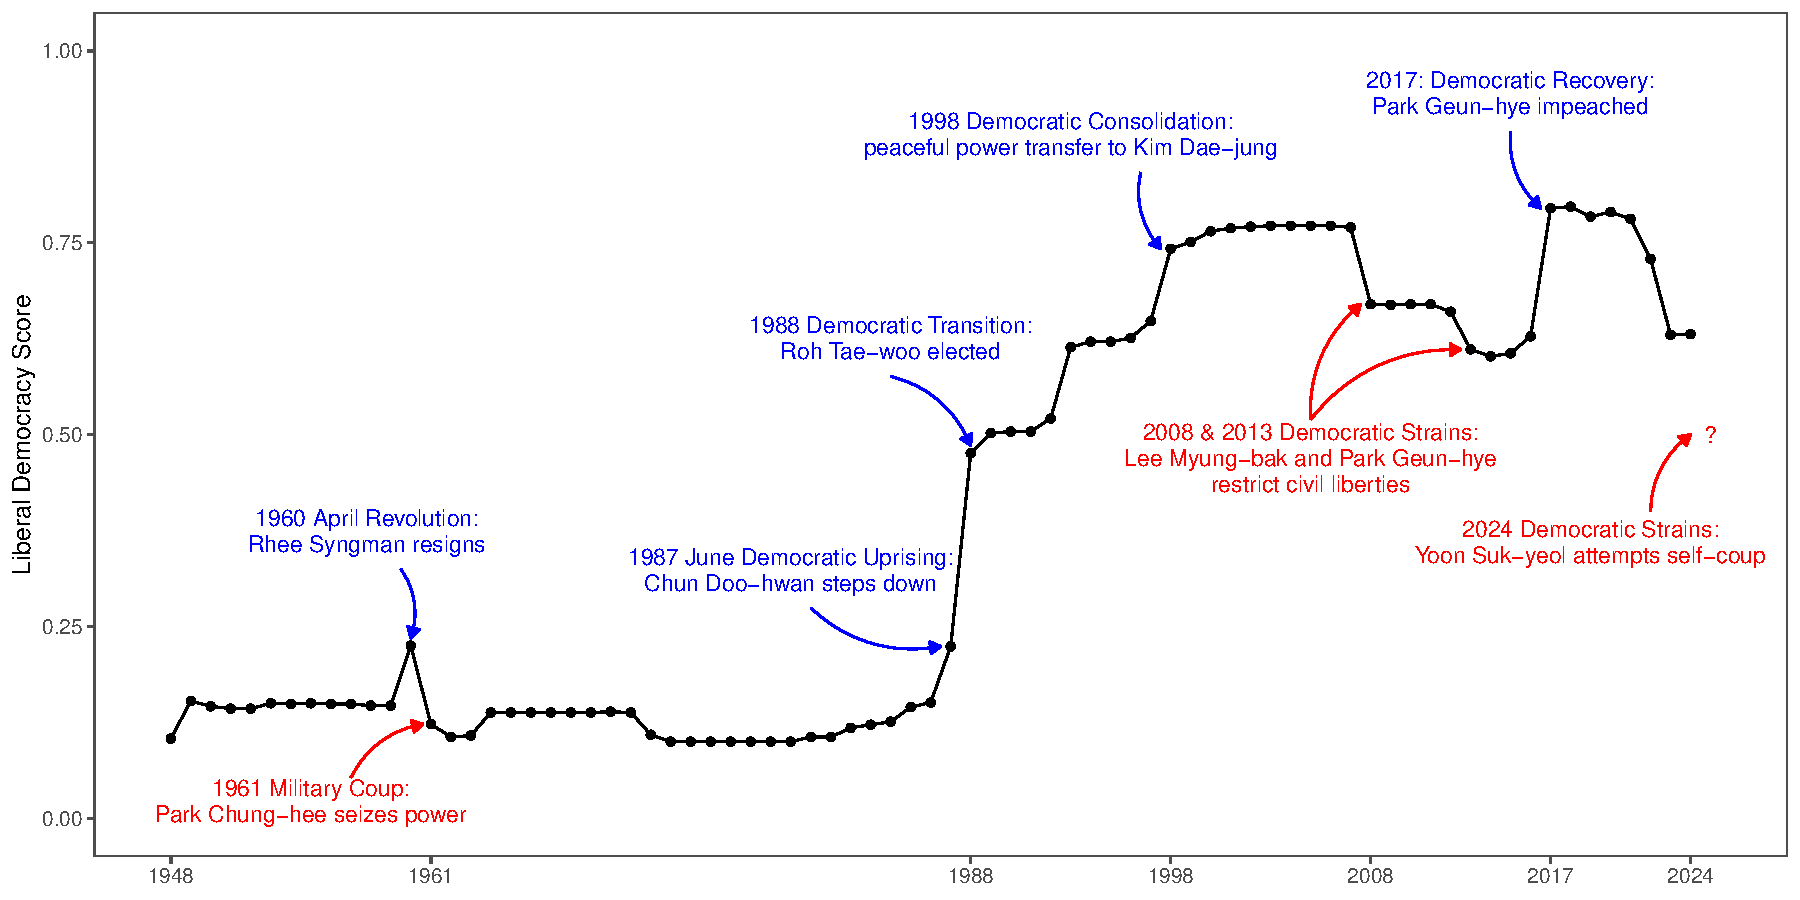
\includegraphics[width=\textwidth]{figures/example.pdf}

  % Caption + note:
  % Many journals prefer tighter line spacing in captions/notes than in body text.
  % Using the 'setspace' package's spacing environment ensures the change is
  % immediate and local (more reliable than changing \baselinestretch).
  \begin{spacing}{1.25}
    \caption{AAA \textit{Note: xxx.}}
    \label{fig:example}
  \end{spacing}

  % Label:
  % - Place after \caption so hyperref links point to the correct anchor.
  % - Keep the label stem consistent with the PDF/TEX stem.
\end{figure}
